\label{game}

In this chapter we want to have the contribution of the human intelligence in making decisions, so we made a simulation game using \textit{Unity}.

%===============================================================================

\section{Introduction to Unity}

Unity is a cross-platform game engine (Fig. \ref{UnityInterface}) developed by Unity Technologies and used to develop video games for PC, consoles, mobile devices and websites. It is a free software (https://unity3d.com/),working with C\# programming language. 
 

\begin{figure}[H]
	\centering
	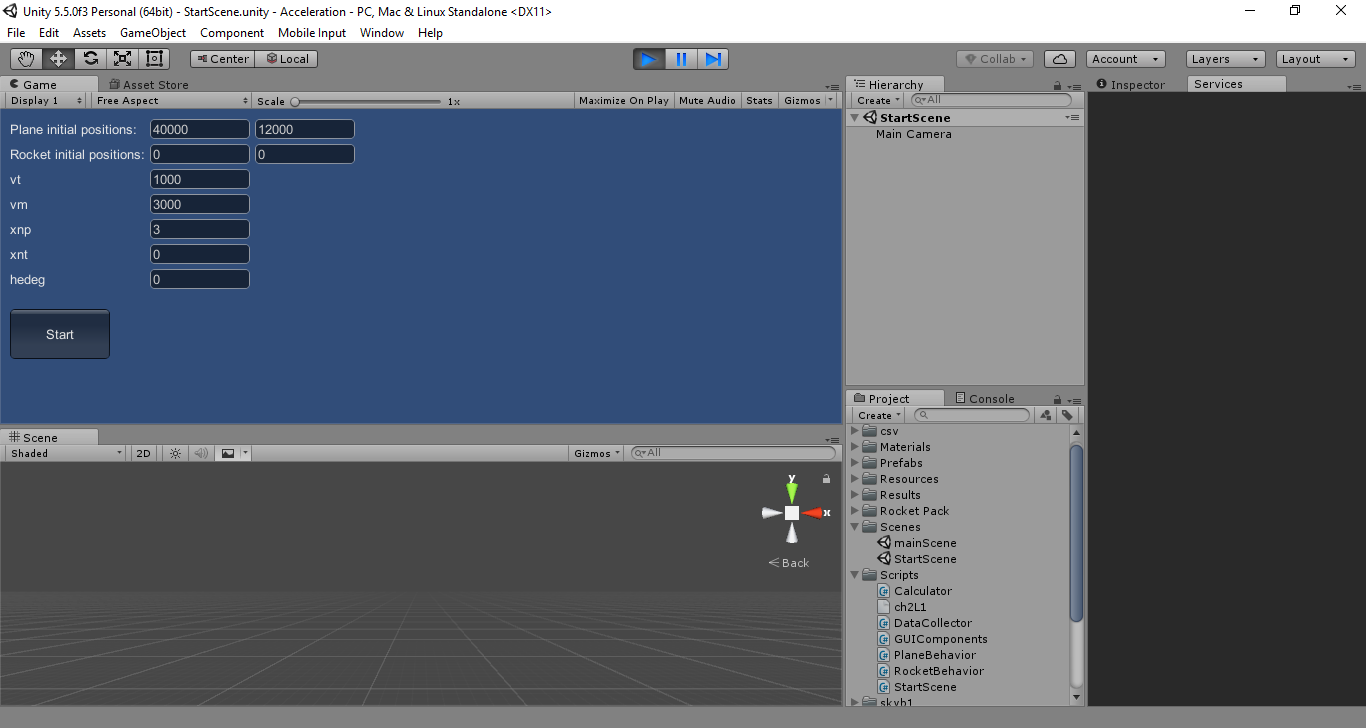
\includegraphics[scale = 0.35]{fig/unityInterface.PNG}
	\caption{Unity game engine interface }
	\label{UnityInterface}
\end{figure}

%===================================================================================

\section{Methodology of the game}

The game (Fig. \ref{UnityGame}) consists of two objects: plane (Target) and missile (Attacker). A human player controls the increasing and decreasing of the target acceleration (XNT) by two arrows on the keyboard. The missile object is moving on according to the proportional navigation guidance law (in sec. \ref{PNeq}).
 
 \begin{figure}[H]
 	\centering
 	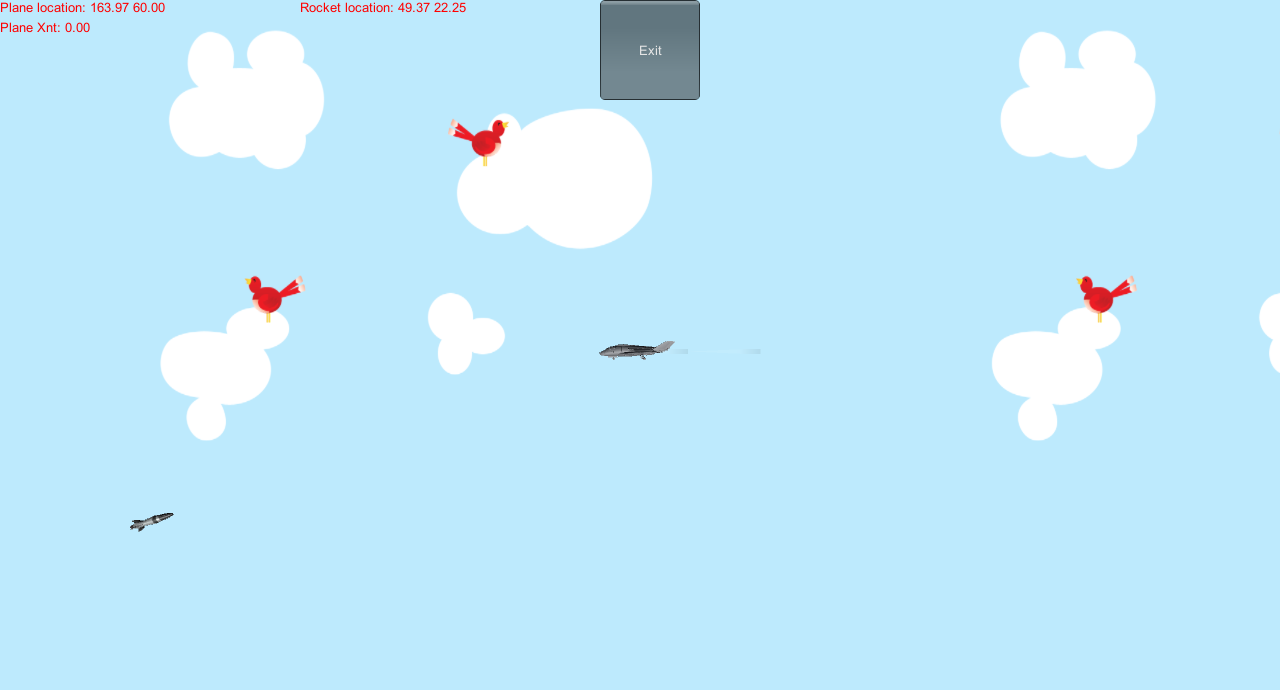
\includegraphics[scale = 0.35]{fig/unityGame.PNG}
 	\caption{Unity game for simulating Target-Attacker engagement}
 	\label{UnityGame}
 \end{figure}
 

%===================================================================================
 
\section{Results}

